
\documentclass[a4paper,10pt]{article}
\usepackage[left=2cm,top=2.5cm,right=2cm]{geometry}
\usepackage[spanish,activeacute]{babel}
\usepackage{caratula}
\usepackage{graphicx}
\usepackage[utf8]{inputenc}
\usepackage{url}
\usepackage{amsmath}
\usepackage{amsfonts}
\usepackage{amssymb} 

 
\parindent = 12 pt
\parskip = 6 pt

\usepackage{fancyhdr}
\usepackage{natbib}
\usepackage{graphicx}

%para agregar el pdf del enunciado en el apendice A
\usepackage{pdfpages}

%encabezado de paginas
\pagestyle{fancy}
\fancyhf{}
\fancyhead [L]{\scriptsize Trabajo Práctico Nº2}
\fancyhead [R]{\scriptsize Giudice, Grenier, Junqueras, Pyrih}
\fancyfoot[C]{\thepage}
\renewcommand{\footrulewidth}{0.4pt} 

\begin{document}

%carátula
\materia{Métodos Numéricos}
\submateria{}
\titulo{Trabajo Práctico Nº2}
\subtitulo{Reconocimiento de caras}
%\grupo{Grupo: GGJP} 
\integrante{Giudice, Carlos}{694/15}{carlosr.giudice@gmail.com}
\integrante{Grenier, Michelle}{418/10}{michelle.grenier@hotmail.com}
\integrante{Junqueras, Juan}{804/16}{juanjunqueras@gmail.com}
\integrante{Pyrih, Franco}{520/12}{fpyrih@dc.uba.ar}
\fecha{Primer cuatrimestre 2018}


\maketitle


\newpage

%índice de contenidos
\tableofcontents


%sección ejemplo, despues la sacamos
%\section{Ejemplo1}
%There is a theory which states that if ever anyone discovers exactly what the %Universe is for and why it is here, it will instantly disappear and be replaced by %something even more bizarre and inexplicable.
%There is another theory which states that this has already happened.\cite{riemann}
%
%\begin{figure}[h!]
%\centering
%\includegraphics[scale=1.7]{universe.jpg}
%\caption{The Universe}
%\label{fig:univerise}
%\end{figure}


%``I always thought something was fundamentally wrong with the universe %2''\citep{burden}\\

%\newpage

%secciones

\clearpage


% from file pautas.pdf:

\section{Resumen} % no más de 200 palabras % son 83



También se llevará a cabo un análisis de la \textit{performance} del algoritmo, teniendo en cuenta tanto el tiempo de cómputo, como la calidad de los resultados que produce.

\paragraph{Palabras clave:} % no más de 4 palabras
Reconocimiento facial, kNN, PCA, validación cruzada
% 


\clearpage

\section{Introducción teórica}

% from file pautas.pdf:

	% Contendrá una breve explicación de la base teórica que fundamenta los métodos involucrados
	% en el trabajo, junto con los métodos mismos. No deben incluirse demostraciones
	% de propiedades ni teoremas, ejemplos innecesarios, ni definiciones elementales (como
	% por ejemplo la de matriz simétrica). En vez de definiciones básicas es conveniente citar
	% ejemplos de bibliografía adecuada. Una cita vale más que mil palabras.




\clearpage

\section{Desarrollo}

% Deben explicarse los métodos numéricos que utilizaron y su aplicación al problema
% concreto involucrado en el trabajo práctico. Se deben mencionar los pasos que si-
% guieron para implementar los algoritmos, las dificultades que fueron encontrando y la
% descripción de cómo las fueron resolviendo. Explicar también cómo fueron planteadas
% y realizadas las mediciones experimentales. Los ensayos fallidos, hipótesis y conjeturas
% equivocadas, experimentos y métodos malogrados deben figurar en esta sección, con
% una breve explicación de los motivos de estas fallas (en caso de ser conocidas).


\subsection{Elección de la estructura de datos}

		

\subsubsection{Implementación}
			

\subsubsection{Planteo de mediciones experimentales}

		
\clearpage

\include{secciones/resultados}
\clearpage

\include{secciones/discusion}
\clearpage

\include{secciones/conclusiones}
\clearpage

\section{Apéndices}

	\subsection{Apéndice A: Enunciado}
	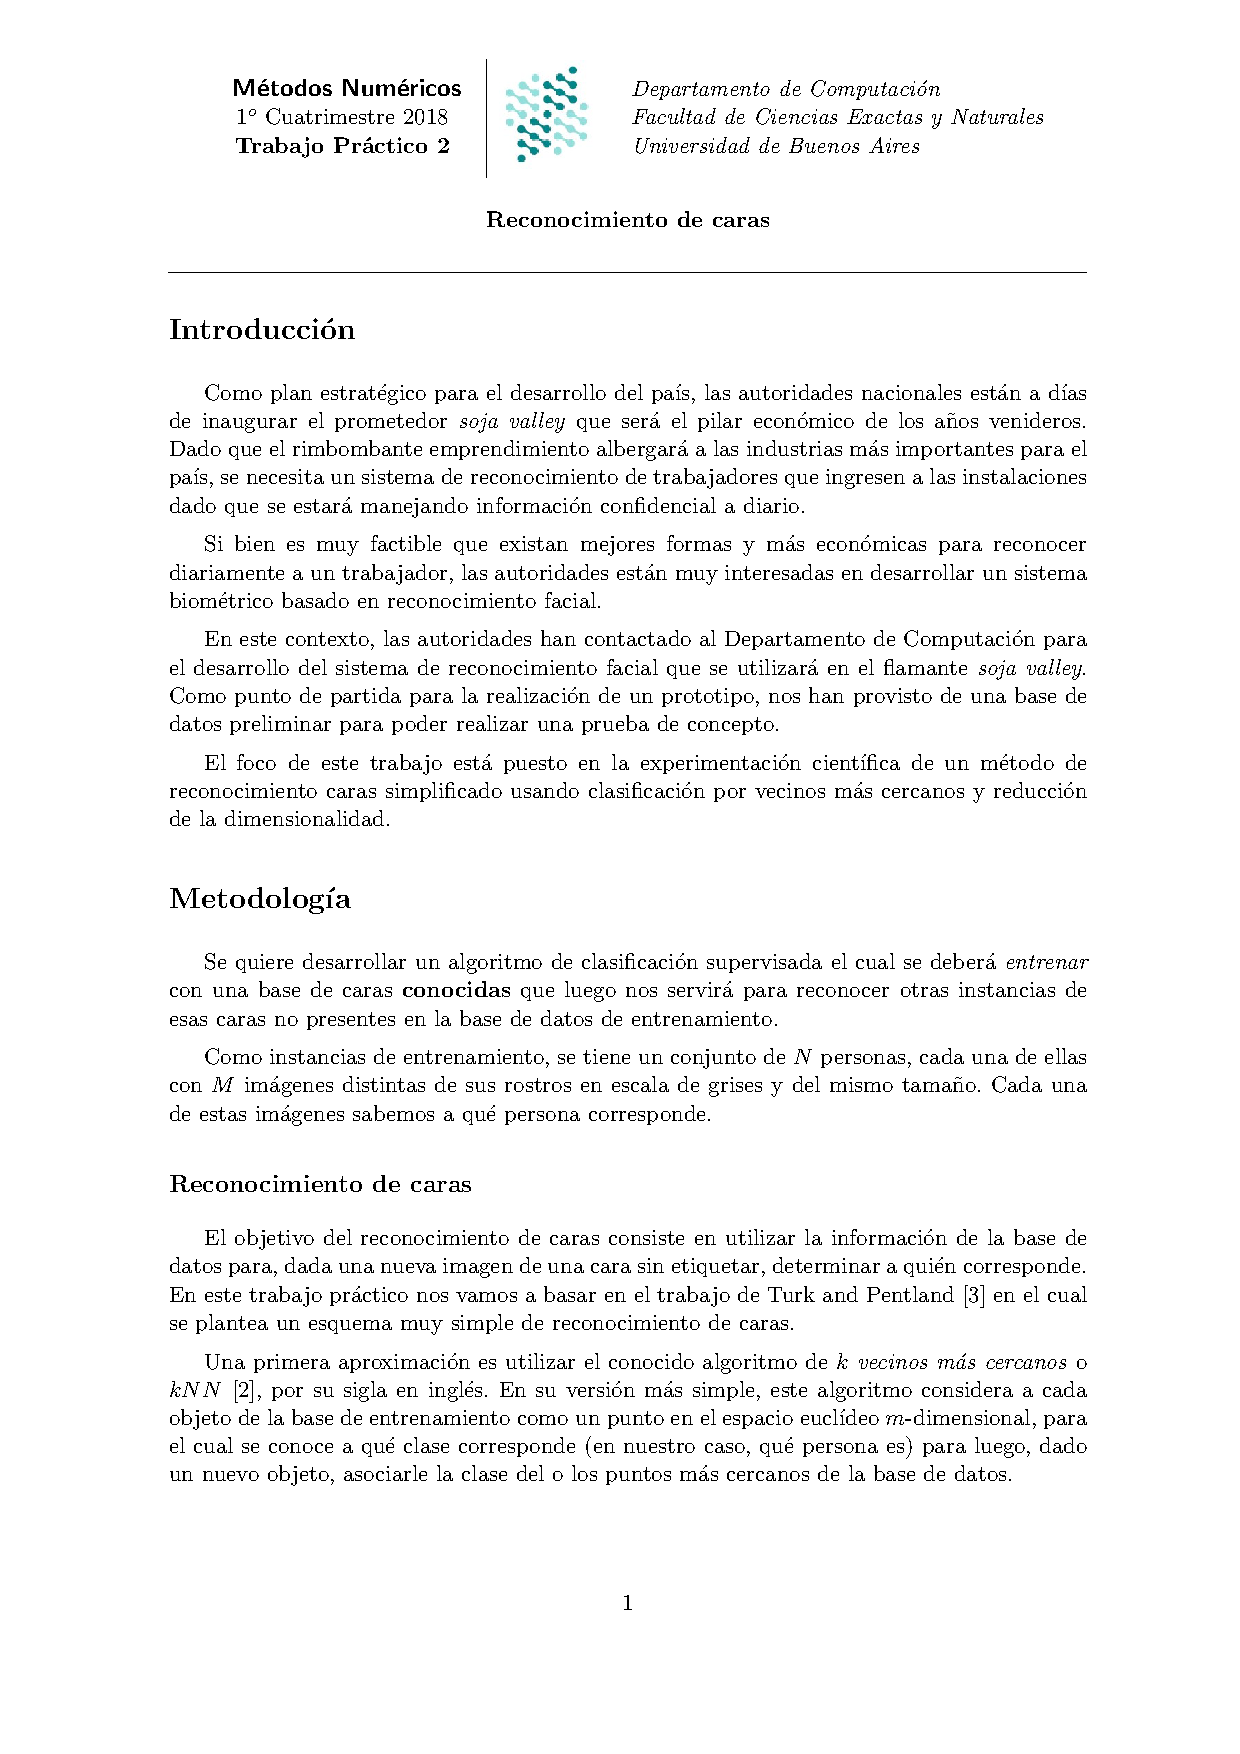
\includepdf[pages=-]{../enunciadoTP2.pdf}
	%\clearpage

	\subsection{Apéndice B: Código fuente numericamente relevante}
	\clearpage

		\subsubsection{\textit{kNN}}

			% \includegraphics[scale=0.75]{img/src/}


		\subsubsection{PCA}

			%\includegraphics[scale=0.6]{img/src/}





	
	\clearpage


\clearpage

\include{secciones/referencias}
\clearpage


\end{document}


